\documentclass[11pt,letterpaper]{article}
\usepackage{fullpage}
\usepackage[pdftex]{graphicx}
\usepackage{amsfonts,eucal,amsbsy,amsopn,amsmath}
\usepackage{url}
\usepackage[sort&compress]{natbib}
\usepackage{natbibspacing}
\usepackage{latexsym}
\usepackage{wasysym} 
\usepackage{rotating}
\usepackage{fancyhdr}
\DeclareMathOperator*{\argmax}{argmax}
\DeclareMathOperator*{\argmin}{argmin}
\usepackage{sectsty}
\usepackage[dvipsnames,usenames]{color}
\usepackage{multicol}
\definecolor{orange}{rgb}{1,0.5,0}
\usepackage{multirow}
\usepackage{sidecap}
\usepackage{caption}
\renewcommand{\captionfont}{\small}
\setlength{\oddsidemargin}{-0.04cm}
\setlength{\textwidth}{16.59cm}
\setlength{\topmargin}{-0.04cm}
\setlength{\headheight}{0in}
\setlength{\headsep}{0in}
\setlength{\textheight}{22.94cm}
\allsectionsfont{\normalsize}
\newcommand{\ignore}[1]{}
\newenvironment{enumeratesquish}{\begin{list}{\addtocounter{enumi}{1}\arabic{enumi}.}{\setlength{\itemsep}{-0.25em}\setlength{\leftmargin}{1em}\addtolength{\leftmargin}{\labelsep}}}{\end{list}}
\newenvironment{itemizesquish}{\begin{list}{\setcounter{enumi}{0}\labelitemi}{\setlength{\itemsep}{-0.25em}\setlength{\labelwidth}{0.5em}\setlength{\leftmargin}{\labelwidth}\addtolength{\leftmargin}{\labelsep}}}{\end{list}}

\bibpunct{(}{)}{;}{a}{,}{,}
\newcommand{\nascomment}[1]{\textcolor{blue}{\textbf{[#1 --NAS]}}}


\pagestyle{fancy}
\lhead{}
\chead{}
\rhead{}
\lfoot{}
\cfoot{\thepage~of \pageref{lastpage}}
\rfoot{}
\renewcommand{\headrulewidth}{0pt}
\renewcommand{\footrulewidth}{0pt}


\title{11-712:  NLP Lab Report}
\author{Jonathan Barker}
\date{April 26, 2013}

\begin{document}
\maketitle
\begin{abstract}
\nascomment{one paragraph here summarizing what the paper is about}
\end{abstract}

\nascomment{brief introduction}

\section{Basic Information about Hindi}
According to \cite{ethnologue}, Hindi (also Khadi Boli or Khari Boli) is an Indo-European language from India that is spoken by 181,676,620 people world-wide. Much of its formal vocabulary comes from Sanskrit. An official language of India, Hindi is a fully developed language written in the Devanagari script.\\
\begin{figure}[h]
  \caption{An example of Devanagri script in a dictionary.}
  \centering
  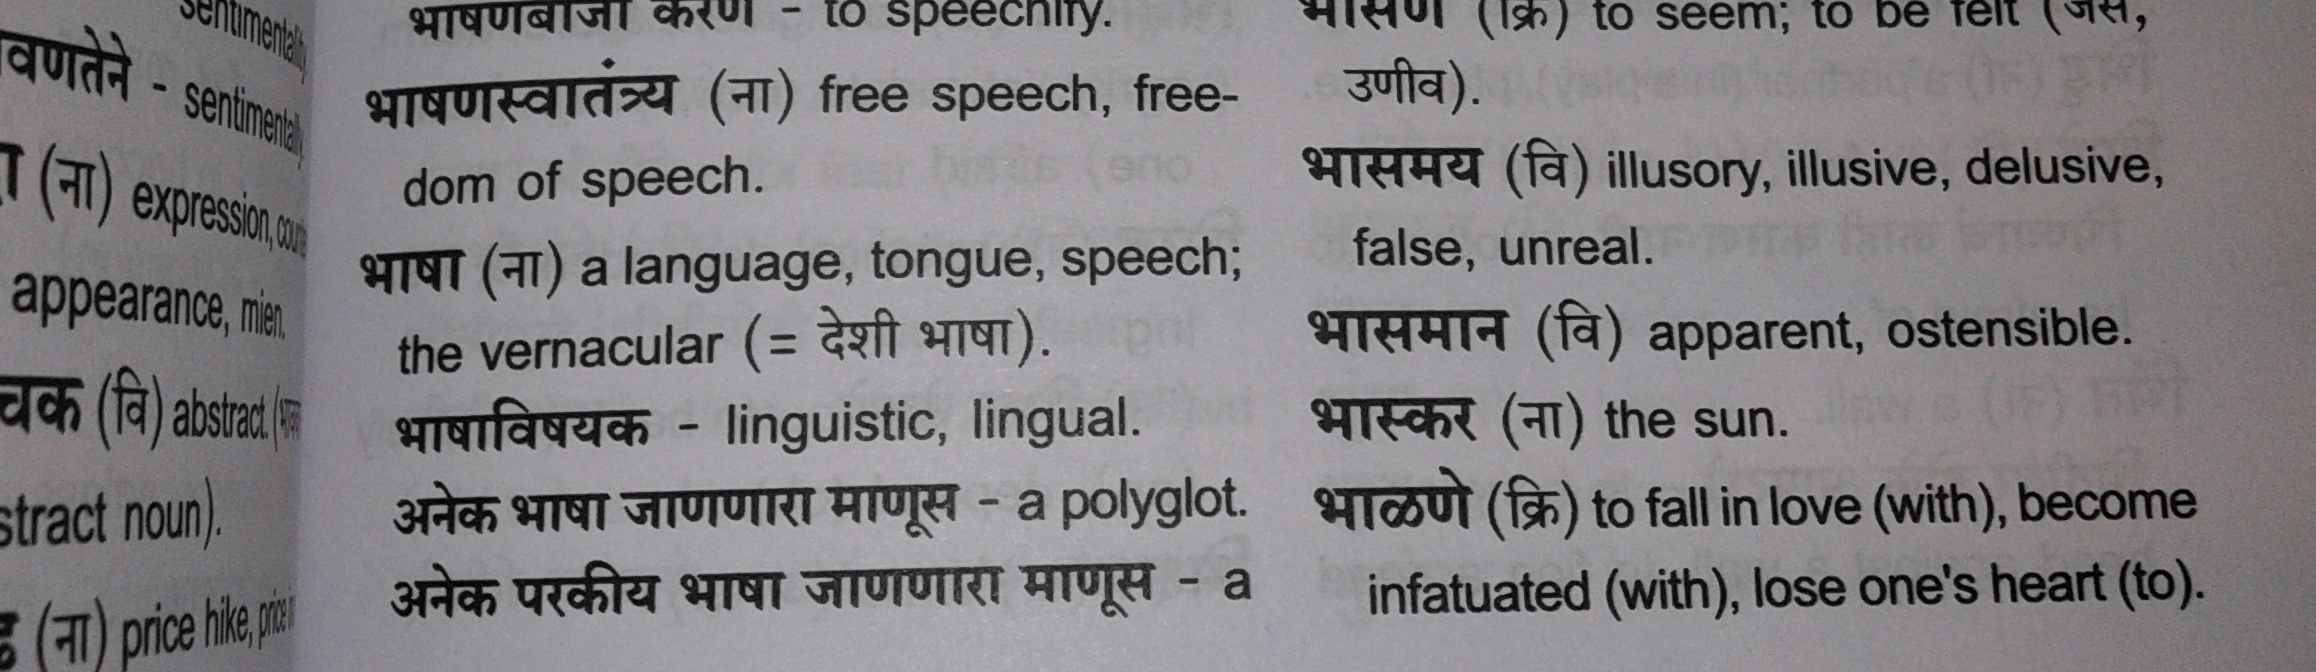
\includegraphics[scale=0.10]{devanagri.jpg}

\end{figure}
\section{Past Work on the Morphology of Hindi}

\section{Available Resources}

\nascomment{include discussion of your corpora}

\section{Survey of Phenomena in Hindi}

\section{Initial Design}

\section{System Analysis on Corpus A}

\section{Lessons Learned and Revised Design}

\section{System Analysis on Corpus B}

\section{Final Revisions}

\section{Future Work}





\bibliographystyle{plainnat}
\bibliography{refs}
\label{lastpage}
\end{document}
